\documentclass[11pt,a4paper]{article}

\usepackage[T1]{fontenc}
\usepackage{lmodern}
\usepackage[margin=2.7cm]{geometry}
\usepackage{amsmath,amssymb,amsthm}
\usepackage{booktabs}
\usepackage{microtype}
\usepackage{tikz}
\usetikzlibrary{patterns}
\usepackage{algorithm}
\usepackage{algpseudocode}
\usepackage{listings}
\usepackage{xcolor}
\usepackage[colorlinks=true,linkcolor=blue!60!black,citecolor=blue!60!black,urlcolor=blue!60!black]{hyperref}

\newtheorem{theorem}{Theorem}
\newtheorem{lemma}{Lemma}
\newtheorem{definition}{Definition}
\newtheorem{observation}{Observation}
\theoremstyle{remark}
\newtheorem{remark}{Remark}

\newcommand{\R}{\mathbb{R}}
\newcommand{\vol}{\operatorname{vol}}
\newcommand{\HV}{\operatorname{HV}}
\newcommand{\Oh}{\mathcal{O}}

\lstset{
  basicstyle=\ttfamily\small,
  keywordstyle=\bfseries,
  commentstyle=\itshape\color{black!60},
  language=Python,
  columns=fullflexible,
  frame=single,
  framerule=0.2pt,
  xleftmargin=1em,
  breaklines=true,
}

\title{Implementation of Chan's Algorithm for Computing the\\ Hypervolume Indicator}
\author{Michael Emmerich\\[2pt] \normalsize University of Jyv\"askyl\"a, Finland}
\date{August 2026}

\begin{document}
\maketitle

\begin{abstract}
The hypervolume indicator, the Lebesgue measure of the region dominated by a
set of $n$ points relative to a reference point in $\R^d$, is a special case of
Klee's measure problem: computing the volume of a union of $n$ axis-parallel
boxes.  Chan's FOCS~2013 paper \emph{``Klee's Measure Problem Made Easy''}
gives (i)~a remarkably simple $\Oh(n^{d/2})$-time algorithm for arbitrary
boxes and (ii)~an $\Oh(n^{d/3}\operatorname{polylog} n)$-time algorithm for
orthants---the case that contains the hypervolume indicator problem.  We
describe complete, self-contained Python implementations of both algorithms;
the second supports orthants of arbitrary orientation, with the grounded
orthants of hypervolume computation as its primary application.  We walk through both algorithms in an implementation-oriented
way, including the symbolic machinery of ``basic functions'' that the
$d/3$-algorithm requires, give a transparent complexity analysis of the code
as written (including where it loses logarithmic factors against the paper's
bounds and why), and validate both implementations exhaustively against
independent exact methods.  Empirically, the recursion-tree size of the
$d/3$-algorithm scales with a visibly smaller exponent than that of the
$d/2$-algorithm, while its symbolic bookkeeping carries large constant
factors; the simple $d/2$-algorithm remains the practical method of choice.
\end{abstract}

\section{Introduction}

Let $Y=\{y_1,\dots,y_n\}\subset\R^d$ be a set of objective vectors (to be
minimized) and let $r\in\R^d$ be a reference point.  The \emph{hypervolume
indicator} of $Y$ is
\begin{equation}
\HV(Y;r) \;=\; \vol\Bigl(\,\bigcup_{i=1}^{n}\,[y_i,r]\,\Bigr),
\qquad [y_i,r] = \{x\in\R^d : y_i \le x \le r\},
\label{eq:hv}
\end{equation}
the volume of the union of the boxes spanned by the points and the reference
point.  It is the most prominent set-quality indicator in evolutionary
multiobjective optimization; it is strictly monotonic with respect to Pareto
dominance and is used both for performance assessment and for selection in
indicator-based algorithms such as SMS-EMOA
\cite{ZitzlerThiele1999,BeumeNaujoksEmmerich2007,GuerreiroFonsecaPaquete2021}.

Equation~\eqref{eq:hv} exhibits the hypervolume indicator as a special case of
\emph{Klee's measure problem} (KMP)~\cite{Klee1977}: given $n$ axis-parallel
boxes in $\R^d$, compute the volume of their union.  The special structure is
that all boxes share the corner $r$; inside the bounding domain each box is a
\emph{grounded orthant} $\{x : x \ge y_i\}$.  Computing the hypervolume
indicator is \#P-hard in $n{+}d$ \cite{BeumeEtAl2009}, so for constant $d$ the
relevant question is the exponent of $n$.

For general KMP, Overmars and Yap's classical algorithm runs in
$\Oh(n^{d/2}\log n)$ time \cite{OvermarsYap1991}; Chan improved this by an
iterated-logarithmic factor \cite{Chan2010} and finally, in the paper this
implementation is based on, to a clean $\Oh(n^{d/2})$ with a strikingly simple
algorithm \cite{Chan2013}.  For the orthant special case, Bringmann's
$\Oh(n^{(d+2)/3})$ algorithm \cite{Bringmann2012} was the first to break the
$d/2$ barrier; Yıldız and Suri gave $\Oh(n^{(d-1)/2}\log n)$ for grounded
boxes \cite{YildizSuri2012}; and Chan's Section~4 achieves the current record,
\begin{equation}
\Oh\bigl(n^{d/3}\operatorname{polylog} n\bigr)\qquad (d\ge 4),
\label{eq:dby3}
\end{equation}
explicitly naming the hypervolume indicator problem as an application.  There
is also good reason to believe the $d/2$ bound for general boxes is
essentially optimal: deciding coverage is W[1]-hard in $d$, and beating
$n^{d/2}$ combinatorially would improve long-standing bounds for
$d$-clique~\cite{Chan2013}.

\paragraph{Contribution.}
This paper documents two self-contained Python implementations
(standard library only):
\begin{itemize}\itemsep2pt
\item \texttt{chan\_hypervolume.py} --- Chan's Section-2 algorithm for
  arbitrary boxes ($\Oh(n^{d/2})$ in the paper; $\Oh(n^{d/2}\log n)$ as
  implemented, see Section~\ref{sec:complexity2}), with a hypervolume
  front end.  To our knowledge this is among the first faithful public
  implementations of the FOCS 2013 algorithm.
\item \texttt{chan\_orthant\_dby3.py} --- Chan's Section-4.2 orthant
  algorithm for orthants of arbitrary orientation (the hypervolume case,
  grounded orthants, is the default front end), including the full symbolic
  ``basic function'' machinery of the paper's Lemmas~4.4 and~4.5.  We are
  not aware of any previous implementation of this algorithm.
\end{itemize}
Section~\ref{sec:simple} walks through the simple algorithm,
Section~\ref{sec:dby3} through the orthant algorithm,
Section~\ref{sec:complexity} gives a transparent complexity analysis of the
implementations as written, and Section~\ref{sec:experiments} reports
validation and scaling experiments.

\paragraph{Conventions.}
Throughout, $d$ is a constant, boxes are axis-parallel, and---following
Chan---all algorithms compute the measure of the \emph{complement} of the
union within a box domain $\Gamma$ (a ``cell''); the union's volume is
recovered as $\vol(\Gamma)$ minus the result.  For hypervolume,
minimization is assumed and the domain is
$\Gamma=[\ell,r]$ with $\ell_k=\min_i (y_i)_k$; each contributing box,
restricted to $\Gamma$, is the grounded orthant $\{x : x\ge y_i\}$.
Dominated points may be discarded beforehand; the implementation does so by
default with an $\Oh(n^2 d)$ prefilter.

\section{The simple $\Oh(n^{d/2})$ algorithm}
\label{sec:simple}

Chan's Section-2 algorithm is a $k$-d-tree-style divide and conquer with one
twist: the input is \emph{simplified} before each cut.

\begin{algorithm}[ht]
\caption{$\textsc{Measure}(B,\Gamma)$ --- measure of $\Gamma\setminus\bigcup B$ \cite{Chan2013}}
\begin{algorithmic}[1]
\State \textbf{if} $|B|$ is below a constant \textbf{then return} the answer directly (inclusion--exclusion)
\State \emph{Simplify} $B$ (eliminate all boxes that are slabs relative to $\Gamma$)
\State \emph{Cut} $\Gamma$ into subcells $\Gamma_L,\Gamma_R$ by a weighted-median hyperplane
\State \textbf{return} $\textsc{Measure}(B|_{\Gamma_L},\Gamma_L)+\textsc{Measure}(B|_{\Gamma_R},\Gamma_R)$
\end{algorithmic}
\label{alg:simple}
\end{algorithm}

\subsection{Step 1: simplification by slab collapse}

Call a box a \emph{slab} (relative to the cell $\Gamma$) if, restricted to
$\Gamma$, it has the form $\{x:\alpha\le x_i\le\beta\}$, i.e.\ it spans
$\Gamma$ in every dimension except $i$.  For each axis $i$, the union of the
slabs of axis $i$ is a union of disjoint intervals in the $x_i$-coordinate;
every point inside them is covered, so they contribute nothing to the
complement.  Chan's elegant elimination is a \emph{monotone re-coordination}:
readjust all $x_i$-values (of the cell and of every box) so that each covered
interval is squeezed to length zero (Figure~\ref{fig:collapse}).  The measure
of the complement is preserved exactly, the slabs disappear, and---the key
structural consequence---\emph{every surviving box now fails to span $\Gamma$
in at least two dimensions}, i.e.\ has a $(d{-}2)$-face intersecting~$\Gamma$.

\begin{figure}[ht]
\centering
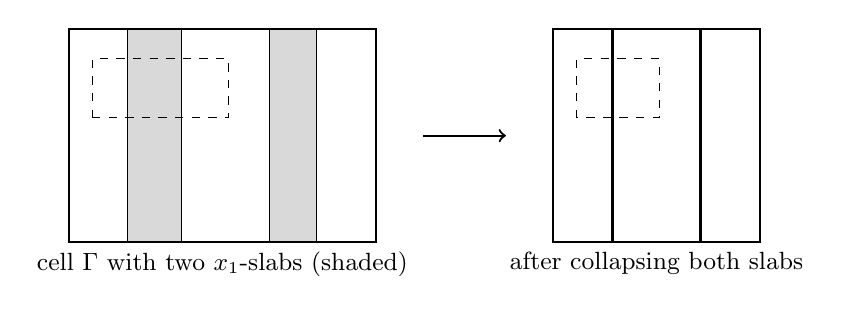
\begin{tikzpicture}[scale=1.5]
  % left: cell with two slabs
  \begin{scope}
    \draw[thick] (0,0) rectangle (2.6,1.8);
    \fill[black!15] (0.5,0) rectangle (0.95,1.8);
    \fill[black!15] (1.7,0) rectangle (2.1,1.8);
    \draw (0.5,0) rectangle (0.95,1.8);
    \draw (1.7,0) rectangle (2.1,1.8);
    \draw[dashed] (0.2,1.05) rectangle (1.35,1.55);
    \node[below] at (1.3,0) {\small cell $\Gamma$ with two $x_1$-slabs (shaded)};
  \end{scope}
  \draw[->,thick] (3.0,0.9) -- (3.7,0.9);
  % right: collapsed
  \begin{scope}[xshift=4.1cm]
    \draw[thick] (0,0) rectangle (1.75,1.8);
    \draw[very thick] (0.5,0) -- (0.5,1.8);
    \draw[very thick] (1.25,0) -- (1.25,1.8);
    \draw[dashed] (0.2,1.05) rectangle (0.9,1.55);
    \node[below] at (0.875,0) {\small after collapsing both slabs};
  \end{scope}
\end{tikzpicture}
\caption{Slab collapse in $d=2$.  The $x_1$-extents covered by slabs are
squeezed to zero width by a monotone map of the $x_1$-axis; the dashed box is
an unaffected input box whose coordinates are pushed through the same map.
The uncovered area is unchanged.}
\label{fig:collapse}
\end{figure}

The implementation (\texttt{\_simplify} + \texttt{\_collapse\_map}) merges the
slab intervals per axis in $\Oh(m\log m)$ time and pushes all coordinates
through the piecewise-linear collapse map.  One subtlety absent from the
paper's one-paragraph description: collapsing axis $i$ can turn a surviving
box into a slab of an axis processed earlier, so the implementation repeats
the sweep until no slabs remain (each extra pass removes at least one box;
see Section~\ref{sec:complexity2}).

\subsection{Step 2: the weighted-median cut}

For a $(d{-}2)$-face orthogonal to axes $i$ and $j$, define its weight as
$2^{(i+j)/d}\in(1,4]$.  The cell is cut by the hyperplane $x_1=m$ where $m$
is the \emph{weighted median} of the first coordinates of the $(d{-}2)$-faces
orthogonal to axis 1 that intersect $\Gamma$.  Then the axes are renumbered
cyclically, $(1,2,\dots,d)\mapsto(d,1,\dots,d-1)$: the cut axis rotates
through the dimensions exactly as in a $k$-d tree.

Why these weights?  Let $N$ denote the total weight of all $(d{-}2)$-faces
intersecting the cell.  After one cut-plus-renumbering:
\begin{itemize}\itemsep1pt
\item a face orthogonal to axes $i,j\neq 1$ keeps its coordinates but its
  weight drops from $2^{(i+j)/d}$ to $2^{(i-1+j-1)/d}$: factor $2^{-2/d}$;
\item a face orthogonal to axes $1,j$ sees its weight \emph{rise} by
  $2^{(d-2)/d}$ under renumbering, but the median cut halves the total weight
  of such faces present in each open subcell: net factor
  $2^{(d-2)/d}/2=2^{-2/d}$.
\end{itemize}
Hence $N$ drops by the factor $2^{2/d}$ in \emph{each} subcell.

\subsection{Analysis}
\label{sec:analysis2}

Writing $T(n,N)$ for the time on inputs with $n$ boxes and total face weight
$N$, simplification gives $T(n,N)\le T(\Oh(N),N)+\Oh(n)$---every surviving box
owns a $(d{-}2)$-face of weight more than 1, so $n=\Oh(N)$ after
simplification---and cutting gives $T(n,N)\le 2\,T(n,N/2^{2/d})+\Oh(n)$.
Combining, with $T(N)=T(cN,N)$:
\begin{equation}
T(N)\;\le\; 2\,T\!\bigl(N/2^{2/d}\bigr)+\Oh(N).
\label{eq:rec2}
\end{equation}
The recursion tree has $2^k$ nodes at level $k$ and reaches constant size at
level $k^\ast=\tfrac d2\log_2 N$, so it has $\Theta(N^{d/2})$ leaves; for
$d\ge 3$ the level costs $2^k\cdot \Oh(N/2^{2k/d})$ grow geometrically
(ratio $2^{1-2/d}>1$), the leaves dominate, and $T(N)=\Oh(N^{d/2})$.  Since
each box has at most $4\binom d2$ faces of weight at most 4,
$N=\Theta(d^2 n)$ and the bound is $\Oh(n^{d/2})$ for constant $d\ge3$.  For
$d=2$ the two terms of \eqref{eq:rec2} balance and all
$\Oh(\log N)$ levels cost $\Oh(N)$: $\Oh(n\log n)$.

\section{The $\Oh(n^{d/3}\operatorname{polylog} n)$ orthant algorithm}
\label{sec:dby3}

For the hypervolume indicator all boxes are grounded orthants, and Chan's
Section~4.2 improves the exponent to $d/3$ by strengthening the
simplification step: besides slabs, it also eliminates all boxes that are
\emph{2-sided orthants} relative to the cell---boxes spanning $\Gamma$ in all
but two dimensions.  After this, every surviving box fails to span $\Gamma$
in at least \emph{three} dimensions, i.e.\ has a $(d{-}3)$-face intersecting
$\Gamma$; cutting at weighted medians of $(d{-}3)$-faces (weight
$2^{(i+j+k)/d}$ for a face orthogonal to axes $i,j,k$, with the same cyclic
renumbering) makes the total face weight decay by $2^{3/d}$ per level, and
the recursion tree shrinks from $\Theta(N^{d/2})$ to $\Theta(N^{d/3})$
leaves.

The price is that 2-sided orthants cannot be eliminated by re-coordination.
Chan's \emph{functional approach} absorbs them into the integrand instead.

\subsection{Basic functions and staircase absorption}
\label{sec:absorb}

\begin{definition}[{Chan \cite[Def.~4.2]{Chan2013}}, adapted]
A \emph{basic function} is a finite sum of terms
\[
c\cdot [E(x)]\cdot h_1(x_1)\cdots h_d(x_d),
\]
where $c\in\R$, each \emph{density} $h_i$ is a univariate step function, and
the \emph{basic predicate} $E$ is a conjunction of $\Oh(d^2)$ conditions of
the form $x_j\le f(x_i)$ or $x_j\ge f(x_i)$ with $f$ a monotone step
function.  Its \emph{complexity} is the total number of pieces of all
functions involved.
\end{definition}

An orthant is given by its vertex $v$ and a sign per axis: the constraint on
axis $k$ is $x_k\ge v_k$ or $x_k\le v_k$.  A constraint is \emph{active} in
the cell $\Gamma$ if its hyperplane actually cuts $\Gamma$.  The recursion
maintains a cell $\Gamma$, a list $\bar B$ of surviving orthants, and a
basic function $F$, and computes
$\int_{\Gamma\setminus\bigcup\bar B} F(x)\,dx$; initially $F\equiv 1$.  The
simplification events are:
\begin{itemize}\itemsep2pt
\item \textbf{Cover.} An orthant with no active constraint covers $\Gamma$:
  the node contributes $0$.
\item \textbf{Slabs.} An orthant with one active constraint is a halfspace;
  its complement chops the cell from one side:
  $\Gamma.\mathrm{hi}_i\leftarrow\min(\Gamma.\mathrm{hi}_i,v_i)$ for a
  $\ge$-constraint, $\Gamma.\mathrm{lo}_i\leftarrow\max(\Gamma.\mathrm{lo}_i,v_i)$
  for a $\le$-constraint; opposing slabs that cross empty the cell.  (For
  orthants no coordinate collapsing is needed---restricted to a cell, a slab
  is always one-sided.)
\item \textbf{2-sided orthants.} The orthants active exactly in dimensions
  $\{i,j\}$ are quadrants in the $(i,j)$-plane, in four orientation classes.
  The complement of the union of each class is a single monotone step
  condition (Figure~\ref{fig:staircase} shows the $(\ge,\ge)$ class):
  \begin{center}
  \begin{tabular}{@{}llll@{}}
  class & covered iff & complement & shape of $f$\\
  $(\ge,\ge)$ & $x_j\ge\min\{b_t: a_t\le x_i\}$ & $x_j\le f(x_i)$ & decreasing\\
  $(\le,\le)$ & $x_j\le\max\{b_t: a_t\ge x_i\}$ & $x_j\ge f(x_i)$ & decreasing\\
  $(\ge,\le)$ & $x_j\le\max\{b_t: a_t\le x_i\}$ & $x_j\ge f(x_i)$ & increasing\\
  $(\le,\ge)$ & $x_j\ge\min\{b_t: a_t\ge x_i\}$ & $x_j\le f(x_i)$ & increasing\\
  \end{tabular}
  \end{center}
  These four staircases are exactly the four monotone boundary functions
  $f^-,g^-,f^+,g^+$ of Chan's Section~4.1.  Absorption multiplies the
  class's condition into every term of $F$; two conditions of the same pair,
  sense, and monotonicity class merge by a pointwise $\min$/$\max$, so the
  predicate size stays $\Oh(d^2)$.
\end{itemize}

\begin{figure}[ht]
\centering
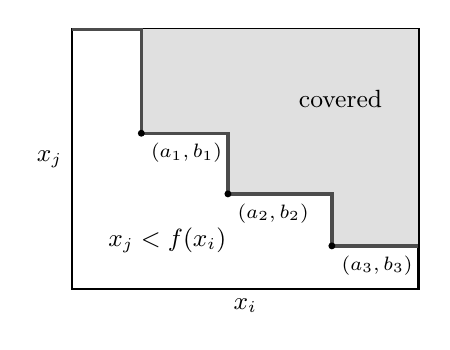
\begin{tikzpicture}[scale=2.2]
  \draw[thick] (0,0) rectangle (2,1.5);
  \fill[black!12] (0.4,0.9) rectangle (2,1.5);
  \fill[black!12] (0.9,0.55) rectangle (2,1.5);
  \fill[black!12] (1.5,0.25) rectangle (2,1.5);
  \draw[very thick] (0,1.5);
  \draw[very thick,black!70]
    (0,1.5) -- (0.4,1.5) -- (0.4,0.9) -- (0.9,0.9) -- (0.9,0.55)
    -- (1.5,0.55) -- (1.5,0.25) -- (2,0.25);
  \fill (0.4,0.9) circle (0.02) node[below right] {\scriptsize $(a_1,b_1)$};
  \fill (0.9,0.55) circle (0.02) node[below right] {\scriptsize $(a_2,b_2)$};
  \fill (1.5,0.25) circle (0.02) node[below right] {\scriptsize $(a_3,b_3)$};
  \node at (1.55,1.1) {\small covered};
  \node at (0.55,0.28) {\small $x_j<f(x_i)$};
  \node[below] at (1,0) {\small $x_i$};
  \node[left] at (0,0.75) {\small $x_j$};
\end{tikzpicture}
\caption{Absorbing 2-sided orthants of a pair $(i,j)$.  The union of the
quadrants (shaded) is bounded by a staircase; the complement is described by
the single condition $x_j<f(x_i)$ with $f$ monotone decreasing---one
condition per orientation class per axis pair, regardless of how many boxes
were absorbed; shown is the $(\ge,\ge)$ class, the other three mirror it.}
\label{fig:staircase}
\end{figure}

\subsection{Symbolic integration (Lemma 4.4)}
\label{sec:lemma44}

The engine underlying everything is one operation: integrate a basic-function
term over one variable $\lambda=x_e$ between a lower bound and an upper
bound.  Every condition touching axis $e$ converts into a bound on $\lambda$:
$[\lambda\le f(x_i)]$ is directly an upper bound, while $[x_j\le f(\lambda)]$
becomes, for monotone $f$, a bound through the \emph{ray preimage}
$\{\lambda: f(\lambda)\ge x_j\}$, whose boundary is a monotone step function
of $x_j$.  This yields upper bounds $U_1,\dots,U_p$ and lower bounds
$V_1,\dots,V_q$, each either a constant or a monotone step function of a
single other variable.  Then, with $h$ the density of axis $e$ and $H$ its
antiderivative,
\[
\int h(\lambda)\prod_t[\lambda\le U_t]\prod_s[\lambda\ge V_s]\,d\lambda
=\Bigl[\max_s V_s\le \min_t U_t\Bigr]\Bigl(H\bigl(\min_t U_t\bigr)-H\bigl(\max_s V_s\bigr)\Bigr).
\]
The implementation performs a case split over which $U_t$ attains the
minimum and which $V_s$ the maximum.  Each guard $[U_t\le U_{t'}]$ is again
expressible in the algebra: trivially true/false for constants, a univariate
indicator folded into a density when both bounds depend on the same variable,
and a new condition $x_b\lessgtr\theta(x_a)$ with
$\theta$ a composed monotone step function otherwise.  Finally
$H\circ(\text{step bound})$ is again a step function, so each case
contributes two new basic-function terms ($+H(U_t)$ and $-H(V_s)$): the class
of basic functions is closed under integration, which is exactly Chan's
Lemma~4.4.  Iterating over all $d$ axes integrates $F$ over a box; this is
the recursion's base case (combined, for up to a constant number of leftover
boxes, with inclusion--exclusion over their intersections, which are boxes).

Two implementation points deserve emphasis:
\begin{itemize}\itemsep2pt
\item \emph{Ties are counted exactly once.}  Bounds are step functions and
  therefore tie on sets of positive measure (plateaus).  The case split uses
  a first-winner rule: candidate $U_t$ wins iff $U_t<U_{t'}$ strictly for all
  $t'<t$ and $U_t\le U_{t'}$ for $t'>t$.  With both strict and non-strict
  guards available, the split partitions the domain up to measure zero.
\item \emph{Plateau preimages are computed from pieces, never by point
  evaluation.}  The preimage of a plateau value under a step function has
  positive measure; all ray preimages and cross-variable comparisons are
  computed exactly from piece values, and point evaluation of a step function
  is only ever applied to raw (Lebesgue) integration variables, where
  breakpoint behaviour is measure-zero.  Everything else in the code may be
  (and is) deliberately sloppy on measure-zero sets, because every predicate
  is ultimately consumed by an integral.
\end{itemize}

\subsection{Compression (Lemma 4.5)}
\label{sec:compress}

Absorbing staircases makes $F$'s complexity grow with the number of absorbed
boxes, which would ruin the recurrence: the problem size passed down must be
proportional to the number of \emph{surviving} boxes.  Chan's fix is to
replace $F$ by its average over the grid spanned by the coordinates of
$\bar B$.  Let $X_i$ be the $x_i$-coordinates appearing among the boxes of
$\bar B$ (plus the cell boundaries), and let $\pi_i^-(x)$ and $\pi_i^+(x)$ be
the grid neighbours of $x$ in $X_i$.  Define
\begin{equation}
\tilde F(x)=\frac{1}{\prod_i\bigl(\pi_i^+(x_i)-\pi_i^-(x_i)\bigr)}
\int_{\pi_1^-(x_1)}^{\pi_1^+(x_1)}\!\!\cdots\int_{\pi_d^-(x_d)}^{\pi_d^+(x_d)}
F(\lambda_1,\dots,\lambda_d)\,d\lambda_d\cdots d\lambda_1 .
\label{eq:avg}
\end{equation}
By construction $\tilde F$ is constant on every grid cell and integrates to
the same value as $F$ over it; since $\bigcup\bar B$ is a union of grid
cells, $\int_{\Gamma\setminus\bigcup\bar B}\tilde F=
\int_{\Gamma\setminus\bigcup\bar B}F$.  Moreover---this is the point---every
occurrence of $x_i$ in \eqref{eq:avg} is filtered through $\pi_i^\pm$, so
every function in $\tilde F$ has breakpoints only on the grid: the complexity
of $\tilde F$ is $\Oh(|\bar B|)$ per function, with $\Oh(1)$ terms (a
constant depending on $d$).

The implementation computes \eqref{eq:avg} with the engine of
Section~\ref{sec:lemma44} verbatim: it renames all variables of $F$ to fresh
integration variables $\lambda_i$, integrates them out one by one with the
\emph{step-function bounds} $\pi_i^-(x_i),\pi_i^+(x_i)$, and multiplies the
reciprocal side lengths into the densities.  A self-test verifies both the
integral-preservation property and the on-grid-breakpoints property on random
instances.  An important soundness detail: all subsequent cuts and
absorptions in the subtree use coordinates of boxes in $\bar B$, which lie on
the grid, so every region over which $\tilde F$ is later integrated remains
grid-aligned---the substitution is valid for the entire subtree, not just for
the current node.

\subsection{The recursion and its analysis}

The driver mirrors Algorithm~\ref{alg:simple} with three changes: absorption
handles covers, slabs, and 2-sided orthants (all cheap; run at every node);
cuts use weighted medians of $(d{-}3)$-face coordinates with weight
$2^{(i+j+k)/d}$ and cyclic renumbering, giving a per-level weight decay of
$2^{3/d}$ by the same argument as in Section~\ref{sec:analysis2}; and
compression, which multiplies the term count by an $\Oh(1)$ factor, is
\emph{throttled}: it runs only every $\approx\log_2(r^d)$ levels.  Grouping
$\log_2(r^d)=d\log_2 r$ consecutive levels into one block, the face weight
decays by $r^3$ per block, the block has $\Oh(r^d)$ subproblems, and one
compression per block restores problem size $\Oh(N)$, giving Chan's
recurrence
\begin{equation}
T(N)\;\le\;\Oh(r^d)\,T\!\bigl(N/r^3\bigr)+\Oh(r^d N).
\label{eq:rec3}
\end{equation}
Choosing $r=N^{\varepsilon}$ for a small constant $\varepsilon>0$ makes the
block depth $1/(3\varepsilon)=\Oh(1)$, so the $\Oh(1)$ compression blowup
multiplies into a constant and \eqref{eq:rec3} solves to
$T(N)=\Oh(N^{d/3}\log^{\Oh(1)}N)$ for $d\ge4$ \cite{Chan2013}.  (For $d=3$
the exponent $d/3=1$ is not interesting: the union of orthants then has
linear complexity anyway.)

\subsection{Scope}

The implementation covers Chan's Section~4.2 in full generality: orthants of
arbitrary orientation, via the four staircase classes of
Section~\ref{sec:absorb} (the general entry point is
\texttt{orthant\_union\_volume}; \texttt{hypervolume\_dby3} is the grounded
front end).  The four classes are exactly the four monotone boundary
functions of the union of $B_{ij}$ in Chan's Section~4.1
\cite[Sec.~4.1]{Chan2013}, and the term algebra treats them uniformly, so
the generalization touches only the absorption front end, the slab handling
(halfspaces now chop the cell from either side, and opposing slabs may empty
it), the active-constraint tests, and the two-sided corners of the
inclusion--exclusion base case.  The paper's further results---the word-RAM
speedups of its Section~3 and the $\Oh(n^{(d+1)/3})$ hypercube algorithm of
its Section~4.3---remain out of scope.

\section{Complexity of the implementations as written}
\label{sec:complexity}

\subsection{\texttt{chan\_hypervolume.py} (Section-2 algorithm)}
\label{sec:complexity2}

\emph{Node count.}  The implementation performs the weighted-median cut
exactly as analyzed, so the recursion tree has $\Oh(N^{d/2})$ nodes with
$N=\Theta(d^2n)$; nothing is lost here.

\emph{Per-node cost.}  With $m$ boxes at a node, clipping is $\Oh(dm)$; one
simplification sweep is $\Oh(d^2m+m\log m)$ (the $\log$ from sorting slab
intervals); collecting cut candidates is $\Oh(d^2 m)$; the weighted median is
computed by sorting, $\Oh(m\log m)$.  The implementation re-sorts at every
node instead of maintaining pre-sorted coordinate lists through the
recursion, and this is precisely where it loses against the paper: summing
level costs as in Section~\ref{sec:analysis2} gives
\begin{equation}
\Oh\bigl(n^{d/2}(d^2+\log n)\bigr)\cdot d^{\Theta(d)}
\qquad\text{for } d\ge 3,
\end{equation}
i.e.\ one extra $\log n$ factor (and $\Oh(n\log^2 n)$ for $d=2$).
Recovering the paper's clean $\Oh(n^{d/2})$ would require threading
pre-sorted per-axis arrays through the recursion and a linear-time weighted
median---both routine, neither affecting the exponent.

\emph{A caveat made explicit.}  The simplification sweep must be iterated
because collapsing axis $i$ can create new slabs on earlier axes.  Each extra
pass removes at least one box, so a node costs at most
$\Oh(d^2m^2)$ in a contrived worst case; across the tree this degrades the
bound to at most $\Oh(n^{d/2+1})$.  We have never observed more than two
passes (one productive, one confirming) in any experiment, and the standard
analysis applies whenever the pass count is $\Oh(1)$ amortized.  \emph{Space}
is linear: the recursion is depth-first and box lists shrink geometrically
along any root--leaf path.

\subsection{\texttt{chan\_orthant\_dby3.py} (Section-4.2 algorithm)}

\emph{Node count.}  Cuts follow the $(d{-}3)$-face weighted-median rule
exactly, so the tree has $\Oh(N_{d-3}^{\,d/3})$ nodes,
$N_{d-3}=\Oh(d^3n)$---this is the quantity the experiments in
Section~\ref{sec:experiments} measure directly.

\emph{Per-node cost.}  Absorption is $\Oh(d^2 m\log m)$.  The dominant cost
is symbolic: integration and compression case-split each term into
$\Oh(pq)$ new terms per eliminated axis ($p,q$ = numbers of upper/lower
bounds, both $\Oh(d)$ after per-pair condition merging), so a single
compression or base-case integration multiplies term counts by a factor that
is bounded for fixed $d$ but grows like $d^{\Theta(d)}$ across the $d$
eliminated axes---Chan's innocuous-looking ``sum of $\Oh(1)$ basic
functions''.  Three measures keep this practical: terms are merged by
structural identity (summing coefficients), dead terms are pruned, and---most
importantly---all functions are restricted to the current cell after every
operation, which trivializes most conditions deep in the tree, where cells
are small.  Compression restores per-function complexity to $\Oh(|\bar B|)$
and is doubly throttled: at least $\max(1,\lceil 0.1\,d\log_2 n\rceil)$
levels between firings (the block schedule of Section~\ref{sec:compress}
with $r=n^{0.1}$), \emph{and} the representation must actually exceed a
constant multiple of its post-compression size $\Oh(d^2|\bar B|)$.  The
second condition matters in practice: for grounded orthants, absorption only
adds or merges conditions and never multiplies the number of terms, so
compression---the sole source of term blowup---should fire only when the
guarantee it provides is actually needed.  (An earlier version of the
implementation compressed on the level schedule alone; on one $d{=}3$,
$n{=}16$ instance this compounded the per-compression blowup into
$9.5\cdot10^4$ terms and a $150$-second running time.  With the size
condition the same instance takes $0.01$ seconds.)

The implementation therefore preserves the $\Theta(N^{d/3})$ recursion-tree
bound while its per-node symbolic overhead contributes polylogarithmic
factors in $n$ with constants that grow steeply in $d$.  This matches the
character of the theoretical result: neither Bringmann's $n^{(d+2)/3}$
algorithm nor Chan's $n^{d/3}$ algorithm was designed for practical constant
factors, and the experiments below confirm that the $d/2$-implementation
dominates in wall-clock time at all reachable input sizes.  The value of the
$d/3$-implementation is as an executable, exhaustively tested reference for
the strongest known hypervolume algorithm.

\section{Validation and experiments}
\label{sec:experiments}

\subsection{Correctness}

Both modules ship with self-tests (run the files directly).  The layered
oracle strategy is worth recording, since the symbolic engine is the kind of
code that is easy to get subtly wrong:
\begin{enumerate}\itemsep2pt
\item \emph{Property tests} for step-function operations, ray preimages
  (including exact plateau levels), and bound comparisons, checked pointwise
  against direct evaluation at thousands of random samples.
\item \emph{Exact integration oracle}: because every function involved is a
  step function, $\int F$ over a box can be computed exactly by enumerating
  the grid of all breakpoints and sampling midpoints; the symbolic engine is
  required to match to $10^{-8}$ relative error on random basic functions in
  $d\le4$ (typical agreement is $10^{-12}$ or better).
\item \emph{Compression oracle}: integral preservation of \eqref{eq:avg}
  over the complement of random orthant unions, plus the structural
  on-grid-breakpoints assertion.
\item \emph{End-to-end}: both algorithms against $\Oh(2^n)$
  inclusion--exclusion for $d\in\{3,4,5\}$, against each other on larger
  random fronts, with compression enabled and disabled, and on
  coordinate-tie-heavy integer grids ($10$ points on a $4^d$ grid), which
  exercise every degenerate branch of the tie handling.  The
  $d/2$-implementation is additionally validated on arbitrary
  (non-orthant) box unions and on spherical fronts against an independent
  coordinate-compression enumerator.  The orthant module is further checked
  on random \emph{mixed-orientation} orthant unions in $d\in\{3,4,5\}$
  (property tests of all four staircase classes, inclusion--exclusion on
  small instances, and the $d/2$-implementation on clipped boxes for up to
  $n=80$), including forced compression.
\end{enumerate}
All checks pass with relative errors at machine-precision level (worst
observed: $4\cdot10^{-14}$).

\subsection{Scaling}

Test instances are \emph{spherical fronts}: $n$ points drawn uniformly by
direction on the positive unit sphere, so that no point dominates another and
nothing can be discarded a priori---the standard hard case for hypervolume
algorithms.  Table~\ref{tab:section2} shows the wall-clock behaviour of the
$d/2$-implementation; empirical exponents are least-squares slopes in
log--log scale.  Real instances sit far below the worst case because
simplification eliminates boxes rapidly.

\begin{table}[ht]
\centering
\caption{\texttt{chan\_hypervolume.py} on spherical fronts (Python 3.13,
one core).  Exponents are empirical fits over the stated $n$-ranges;
theoretical worst-case node exponent is $d/2$.}
\label{tab:section2}
\begin{tabular}{@{}rrrrrr@{}}
\toprule
$d$ & $n$-range & nodes $\sim n^{x}$ & time $\sim n^{x}$ & worst-case $x$ & largest run \\
\midrule
2 & 64--1024 & 1.02 & 1.20 & 1.0 & $n{=}1024$: 0.07\,s\\
3 & 50--800  & 1.04 & 1.31 & 1.5 & $n{=}800$: 0.25\,s\\
4 & 25--400  & 1.33 & 1.43 & 2.0 & $n{=}400$: 0.50\,s\\
5 & 25--200  & 1.68 & 1.84 & 2.5 & $n{=}200$: 1.34\,s\\
6 & 20--80   & 2.28 & 2.43 & 3.0 & $n{=}80$: 1.51\,s\\
\bottomrule
\end{tabular}
\end{table}

\begin{table}[ht]
\centering
\caption{Recursion-tree size, $d/2$- vs.\ $d/3$-algorithm, same spherical-front
instances (reference point $1.2\cdot\mathbf 1$).  ``exp'' is the empirical
node-count exponent; predicted worst-case exponents are $d/2$ and $d/3$.
Wall-clock times illustrate the symbolic overhead of the $d/3$ algorithm.}
\label{tab:compare}
\begin{tabular}{@{}rrrrrrrr@{}}
\toprule
& & \multicolumn{2}{c}{node exponent} & \multicolumn{2}{c}{nodes at largest $n$} & \multicolumn{2}{c}{time at largest $n$}\\
\cmidrule(lr){3-4}\cmidrule(lr){5-6}\cmidrule(l){7-8}
$d$ & $n$-range & $d/2$-alg & $d/3$-alg & $d/2$-alg & $d/3$-alg & $d/2$-alg & $d/3$-alg\\
\midrule
3 & 16--256 & 1.21 & 1.12 & 1267 & 251 & 0.07\,s & 0.13\,s\\
4 & 12--96  & 1.70 & 1.49 & 2485 & 545 & 0.12\,s & 0.49\,s\\
5 & 8--32   & 2.18 & 1.70 & 1823 & 393 & 0.08\,s & 0.50\,s\\
\bottomrule
\end{tabular}
\end{table}

Table~\ref{tab:compare} compares the two recursion trees on identical
instances.  The $d/3$-algorithm's tree is consistently a factor 4--5 smaller
and grows with a visibly smaller exponent---the theoretical improvement is
measurable in exactly the quantity the analysis bounds.  Its wall-clock time
is nevertheless $2$--$7\times$ higher at these sizes: the per-node work
(staircase construction, condition merging, pruning, symbolic base-case
integration) outweighs the smaller tree.  Notably, on these instances the
adaptive throttle never needs to fire a compression and the basic function
stays a single term throughout; when compression is \emph{forced} to fire
(e.g.\ every 3 levels with a zero size threshold), results are unchanged but
term counts reach the hundreds and running time grows sharply---consistent
with the analysis, which permits only $\Oh(1)$ compressions per root--leaf
path.  Both implementations agree to at least $10^{-8}$ relative error on
every instance.

\section{Usage}

\begin{lstlisting}
from chan_hypervolume import hypervolume            # O(n^{d/2} log n), practical
from chan_orthant_dby3 import hypervolume_dby3      # O(n^{d/3} polylog n), reference

points = [(0.2, 0.7, 0.3), (0.5, 0.2, 0.6), (0.8, 0.4, 0.1)]
ref    = (1.0, 1.0, 1.0)          # minimization; use maximize=True otherwise

hv  = hypervolume(points, ref)
hv3 = hypervolume_dby3(points, ref)   # identical value, d >= 3 only
\end{lstlisting}

\noindent Both functions accept \texttt{maximize=True} and
\texttt{prefilter=False}; the general Klee's-measure entry point
\texttt{union\_volume(boxes)} in \texttt{chan\_hypervolume.py} accepts
arbitrary boxes as \texttt{(lo, hi)} corner pairs, and
\texttt{orthant\_union\_volume(orthants, lo, hi)} in
\texttt{chan\_orthant\_dby3.py} accepts arbitrary-orientation orthants as
\texttt{(vertex, signs)} pairs measured inside a domain box.  The solver classes
(\texttt{ChanMeasure}, \texttt{ChanOrthantMeasure}) expose node counts and,
for the latter, the compression interval and a switch to disable compression.

\section{Conclusions}

Chan's ``easy'' algorithm fully lives up to its name: the $d/2$
implementation is under 300 lines of executable logic, uses no data structure
beyond sorted lists, and computes exact hypervolumes of fronts with hundreds
of points in seconds up to $d=7$.  The $d/3$ orthant algorithm is a different
kind of object: its recursion is just as simple, but the basic-function
algebra it stands on---closure of step-function predicates under
integration, and grid-averaging compression---is intricate to implement
correctly, chiefly because of positive-measure ties between step functions.
We believe the implementation presented here is the first of that algorithm;
its recursion-tree scaling matches the $d/3$ theory, and it provides an
executable specification against which faster engineered variants (or an
implementation of the hypercube case) can be checked.

\paragraph{Code availability.}
Both modules, the test suites, and the benchmark scripts are available in the
accompanying repository (\texttt{FastHVChan}); everything depends only on the
Python standard library.

\paragraph{Acknowledgements.}
The implementations and this manuscript were co-created by the author and
Claude Fable~5 (Anthropic) in an interactive agentic coding session, working
directly from Chan's paper \cite{Chan2013}.

\begin{thebibliography}{10}\setlength{\itemsep}{2pt}

\bibitem{Klee1977}
V.~Klee.
\newblock Can the measure of $\bigcup[a_i,b_i]$ be computed in less than
  $O(n\log n)$ steps?
\newblock \emph{American Mathematical Monthly}, 84:284--285, 1977.

\bibitem{OvermarsYap1991}
M.~H. Overmars and C.-K. Yap.
\newblock New upper bounds in Klee's measure problem.
\newblock \emph{SIAM Journal on Computing}, 20(6):1034--1045, 1991.

\bibitem{Chan2010}
T.~M. Chan.
\newblock A (slightly) faster algorithm for Klee's measure problem.
\newblock \emph{Computational Geometry: Theory and Applications},
  43(3):243--250, 2010.

\bibitem{Chan2013}
T.~M. Chan.
\newblock Klee's measure problem made easy.
\newblock In \emph{Proc.\ 54th IEEE Symposium on Foundations of Computer
  Science (FOCS)}, pages 410--419, 2013.

\bibitem{Bringmann2012}
K.~Bringmann.
\newblock An improved algorithm for Klee's measure problem on fat boxes.
\newblock \emph{Computational Geometry: Theory and Applications},
  45(5--6):225--233, 2012.

\bibitem{YildizSuri2012}
H.~Y{\i}ld{\i}z and S.~Suri.
\newblock On Klee's measure problem for grounded boxes.
\newblock In \emph{Proc.\ 28th ACM Symposium on Computational Geometry
  (SoCG)}, pages 111--120, 2012.

\bibitem{ZitzlerThiele1999}
E.~Zitzler and L.~Thiele.
\newblock Multiobjective evolutionary algorithms: A comparative case study
  and the strength {P}areto approach.
\newblock \emph{IEEE Transactions on Evolutionary Computation},
  3(4):257--271, 1999.

\bibitem{BeumeNaujoksEmmerich2007}
N.~Beume, B.~Naujoks, and M.~Emmerich.
\newblock {SMS-EMOA}: Multiobjective selection based on dominated
  hypervolume.
\newblock \emph{European Journal of Operational Research},
  181(3):1653--1669, 2007.

\bibitem{BeumeEtAl2009}
N.~Beume, C.~M. Fonseca, M.~L{\'o}pez-Ib{\'a}{\~n}ez, L.~Paquete, and
  J.~Vahrenhold.
\newblock On the complexity of computing the hypervolume indicator.
\newblock \emph{IEEE Transactions on Evolutionary Computation},
  13(5):1075--1082, 2009.

\bibitem{WhileEtAl2006}
L.~While, P.~Hingston, L.~Barone, and S.~Huband.
\newblock A faster algorithm for calculating hypervolume.
\newblock \emph{IEEE Transactions on Evolutionary Computation},
  10(1):29--38, 2006.

\bibitem{GuerreiroFonsecaPaquete2021}
A.~P. Guerreiro, C.~M. Fonseca, and L.~Paquete.
\newblock The hypervolume indicator: Computational problems and algorithms.
\newblock \emph{ACM Computing Surveys}, 54(6):119:1--119:42, 2021.

\bibitem{PatersonYao1992}
M.~S. Paterson and F.~F. Yao.
\newblock Optimal binary space partitions for orthogonal objects.
\newblock \emph{Journal of Algorithms}, 13(1):99--113, 1992.

\end{thebibliography}

\end{document}
